
\let\negmedspace\undefined
\let\negthickspace\undefined
\documentclass[journal]{IEEEtran}
\usepackage[a5paper, margin=10mm, onecolumn]{geometry}
%\usepackage{lmodern} % Ensure lmodern is loaded for pdflatex
\usepackage{tfrupee} % Include tfrupee package
\setlength{\headheight}{1cm} % Set the height of the header box
\setlength{\headsep}{0mm}     % Set the distance between the header box and the top of the text
\usepackage{gvv-book}
\usepackage{gvv}
\usepackage{cite}
\usepackage{amsmath,amssymb,amsfonts,amsthm}
\usepackage{algorithmic}
\usepackage{graphicx}
\usepackage{textcomp}
\usepackage{xcolor}
\usepackage{txfonts}
\usepackage{listings}
\usepackage{enumitem}
\usepackage{mathtools}
\usepackage{gensymb}
\usepackage{comment}
\usepackage[breaklinks=true]{hyperref}
\usepackage{tkz-euclide} 
\usepackage{listings}
% \usepackage{gvv}                                        
\def\inputGnumericTable{}                                 
\usepackage[latin1]{inputenc}                                
\usepackage{color}                                            
\usepackage{array}                                            
\usepackage{longtable}                                       
\usepackage{calc}                                             
\usepackage{multirow}                                         
\usepackage{hhline}                                           
\usepackage{ifthen}                                           
\usepackage{lscape}
\renewcommand{\thefigure}{\theenumi}
\renewcommand{\thetable}{\theenumi}
\setlength{\intextsep}{10pt} % Space between text and floats
\numberwithin{equation}{enumi}
\numberwithin{figure}{enumi}
\renewcommand{\thetable}{\theenumi}
\begin{document}
\bibliographystyle{IEEEtran}
\title{11.16.3.7}
\author{EE24BTECH11041 - Mohit}
% \maketitle
% \newpage
% \bigskip
{\let\newpage\relax\maketitle}
\textbf{Question:-} A fair coin is tossed four times, and a person wins Rs.1 for each head and loses Rs.1.50 for each tail. From the sample space, calculate how many different amounts of money you can have after four tosses and the probability of having each of these amounts.

\textbf{Solution}

Let:
\begin{align}
H = +1 \quad \text{(gain Rs.1 for Head)}, \quad T = -1.50 \quad \text{(lose Rs.1.50 for Tail)}.
\end{align}

For $ x $, the number of heads in 4 tosses, the total net money can be calculated using the formula:
\begin{align}
\text{Net Money} = x(1) + (4-x)(-1.5)\\
\text{Net Money} = x - 1.5(4-x)\\
\text{Net Money} = 2.5x - 6,
\end{align}

where $ x = 0, 1, 2, 3, 4 $.

\textbf{Possible Outcomes and Net Money}

\begin{itemize}
    \item $ x = 0 $: All tails ($ TTTT $):
    \begin{align}
    \text{Net Money} = 2.5(0) - 6 = -6
    \end{align}
    \item $ x = 1 $: One head, three tails ($ HTTT, THTT, TTHT, TTTH $, etc.):
    \begin{align}
    \text{Net Money} = 2.5(1) - 6 = -3.5
    \end{align}
    \item $ x = 2 $: Two heads, two tails ($ HHTT, HTHT, HTTH, \dots $):
    \begin{align}
    \text{Net Money} = 2.5(2) - 6 = -1
    \end{align}
    \item $ x = 3 $: Three heads, one tail ($ HHHT, HHTH, HTHH, THHH $):
    \begin{align}
    \text{Net Money} = 2.5(3) - 6 = 1.5
    \end{align}
    \item $ x = 4 $: All heads ($ HHHH $):
    \begin{align}
    \text{Net Money} = 2.5(4) - 6 = 4
    \end{align}
\end{itemize}

\textbf{Number of Outcomes for Each Case}

The number of outcomes for each $ x $ is given by the binomial coefficient $ \binom{4}{x} $:

\begin{align}
    &x = 0: \binom{4}{0} = 1, \\
    &x = 1: \binom{4}{1} = 4, \\
    &x = 2: \binom{4}{2} = 6, \\
    &x = 3: \binom{4}{3} = 4, \\
    &x = 4: \binom{4}{4} = 1
\end{align}

\textbf{Probabilities of Each Case}

Since the coin is fair, the probability of each outcome is $ \frac{1}{16} $. The probabilities for each $ x $ are:

\begin{align}
    &x = 0: \text{Probability} = \frac{\binom{4}{0}}{16} = \frac{1}{16}, \\
    &x = 1: \text{Probability} = \frac{\binom{4}{1}}{16} = \frac{4}{16} = \frac{1}{4}, \\
    &x = 2: \text{Probability} = \frac{\binom{4}{2}}{16} = \frac{6}{16} = \frac{3}{8}, \\
    &x = 3: \text{Probability} = \frac{\binom{4}{3}}{16} = \frac{4}{16} = \frac{1}{4}, \\
    &x = 4: \text{Probability} = \frac{\binom{4}{4}}{16} = \frac{1}{16}.
\end{align}


\textbf{CODING LOGIC:-}


\textbf{Bernoulli Random Variable for Coin Toss}\\
Let the outcome of each coin toss be represented by a Bernoulli random variable \( X \), where:

\[
X = 
\begin{cases} 
1 & \text{if the toss is a head (H)} \\
0 & \text{if the toss is a tail (T)}
\end{cases}
\]

Since the coin is fair, the probability of getting heads or tails is:

\begin{align}
  p_X\brak{x} = \begin{cases}
    \frac{1}{2} & x = 0\\
    \frac{1}{2} & x = 1
  \end{cases}
\end{align}
\textbf{Finding the \( z \)-Transform of a Single Toss}

The moment generating function (MGF) for one coin toss \( X_i \) is:
\begin{align}
M_{X_i}(z) = \sum_{k=-\infty}^{\infty} p_{X_i}(n) z^{-k}
\end{align}

Since \( X_i \) takes values 0 and 1, we sum over these cases:
\begin{align}
M_{X_i}(z) = p z^{-1} + (1 - p)
\end{align}

For a fair coin where \( p = 0.5 \), this simplifies to:
\begin{align}
M_{X_i}(z) = 0.5z^{-1} + 0.5
\end{align}

\textbf{Extending to 4 Tosses (Binomial Distribution)}

Since the total number of heads in 4 tosses follows a binomial distribution, the moment generating function for \( X \) is:
\begin{align}
M_X(z) = \prod_{i=1}^{4} M_{X_i}(z) \\
M_X(z) = \left( 0.5z^{-1} + 0.5 \right)^4
\end{align}

\textbf{Step 4: Expanding Using Binomial Theorem}

Using the binomial theorem:
\begin{align}
(a + b)^n = \sum_{k=0}^{n} \binom{n}{k} a^k b^{n-k}
\end{align}
where \( a = 0.5z^{-1} \) and \( b = 0.5 \), we get:
\begin{align}
M_X(z) = \sum_{k=0}^{4} \binom{4}{k} (0.5)^4 z^{-k}
\end{align}

Since \( (0.5)^4 = \frac{1}{16} \), we simplify:
\begin{align}
M_X(z) = \sum_{k=0}^{4} \binom{4}{k} \frac{z^{-k}}{16}
\end{align}

Expanding the binomial coefficients:
\begin{align}
M_X(z) = \frac{1}{16} \left( z^{-0} + 4z^{-1} + 6z^{-2} + 4z^{-3} + z^{-4} \right) \\
M_X(z) = \frac{1}{16} + \frac{4}{16}z^{-1} + \frac{6}{16}z^{-2} + \frac{4}{16}z^{-3} + \frac{1}{16}z^{-4}
\end{align}

The coefficient of \( z^{-k} \) gives the probability \( P(X = k) \), which corresponds to the binomial probability mass function (PMF):
\begin{align}
P(X = k) = \binom{4}{k} (0.5)^4
\end{align}

\textbf{Money Calculation}

Let \( M(k) \) represent the total amount of money after \( k \) heads. The money is calculated as:
\begin{align}
M(k) = 2.5k - 6
\end{align}
where \( k \) is the number of heads. The possible amounts of money are:
\begin{itemize}
    \item For \( k = 0 \): \( M(0) = -6 \)
    \item For \( k = 1 \): \( M(1) = -3.5 \)
    \item For \( k = 2 \): \( M(2) = -1 \)
    \item For \( k = 3 \): \( M(3) = 1.5 \)
    \item For \( k = 4 \): \( M(4) = 4 \)
\end{itemize}
\textbf{PMF for Money \( M(k) \)}

\begin{itemize}
    \item \( P(M = -6) = P(X = 0) = \frac{1}{16} \)
    \item \( P(M = -3.5) = P(X = 1) = \frac{4}{16} \)
    \item \( P(M = -1) = P(X = 2) = \frac{6}{16} \)
    \item \( P(M = 1.5) = P(X = 3) = \frac{4}{16} \)
    \item \( P(M = 4) = P(X = 4) = \frac{1}{16} \)
\end{itemize}

 \textbf{CDF for Money \( M(k) \)}

\begin{align}
P(M \leq -6) = P(X = 0) = \frac{1}{16} \\
P(M \leq -3.5)   = \frac{5}{16}\\
P(M \leq -1)  = \frac{11}{16}\\
P(M \leq 1.5) =  \frac{15}{16}\\
P(M \leq 4)  = 1
\end{align}


\begin{figure}[h!]
   \centering
   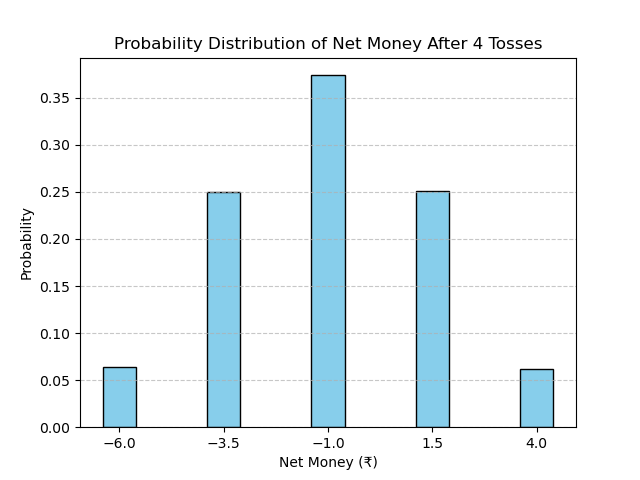
\includegraphics[width=0.7\linewidth]{figs/Figure_1.png}
\end{figure}

\end{document}
